%////////////////////////////////////////////////
% ToDo:
% Einleitung mit Use-Cases
% Beispiele!
% Grobe Use-Cases
% Use-Cases erklären
%////////////////////////////////////////////////

\chapter{Conceptual Design}
\label{chap:conceptual-design}
The goal of this thesis is to develop a system that allows generating large sets of images for training neural networks. As this environment shall be used as a drop-in replacement for conventional methods such as taking photos and labeling those by hand, the generated images must be of excellent quality and labeled.\\
This chapter will introduce the terminology, central ideas and architectural basics of a concept that can be used for implementation by explaining its high-level features using use-cases, refining those to specific user-interactions and deducing components from them.

%////////////////////////////////////////////////
\section{System Environment and Terminology}
%\begin{wrapfigure}{R}{0.4\textwidth}
%\centering
%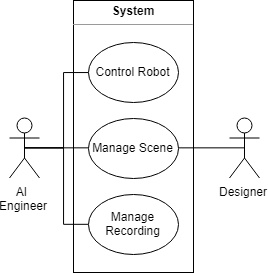
\includegraphics[width=0.4\textwidth]{tex/img/ch04/Use_Cases_06.png}
%\caption{\label{fig:use-cases-abstract}Abstract Use-Cases}
%\end{wrapfigure}
% *** Scenes
The system features at least one virtual 3D environment (a \textit{scene}) that represents a specific place (either an existing or non-existing place) and a virtual robot that operates in said environment. It is used by two groups of users: \textit{designers} and \textit{\ac{AI} engineers}. Figure \ref{fig:use-cases-abstract} shows these groups of users and their high-level and abstract use-cases.\\
% *** Robots
A virtual \textit{robot} is a representation of a real or fictional robot. It is mainly used to navigate a virtual camera used for capturing records from the robot's perspective while its movement is restricted by its body's specifics (considering different types of drives such as limbs or wheels and their respective attributes such as degrees of freedom or torque).\\
% *** Designers
Scenes need to be created, populated and configured. \textit{Designers} set up scenes so that they can be used in a production environment. They recreate existing or non-existing places by adding 3D objects and light-sources to scenes. Depending on the specific use of the scene and individual objects in it, designers can add \textit{mutators} to any entities in a scene and equip them with an initial configuration. They can also add waypoints to the scene for allow robots to travel along paths.\\
% *** AI engineers
\textit{\acs{AI} engineers} use the system to capture records. To do so they can use the system in one of two modes: \textit{"manual control"} lets them take control of robots and maneuver them in scenes, textit{"automatic mode"} allows them to let robots travel along preconfigured paths. At any time they can toggle automatic capture and labeling of images and activity of mutators.\\
% *** Records
A \textit{record} is a data-structure that contains an image and meta-data about the image, such as the location and view-angles of the camera at the time of capturing the image and a list of labels. \textit{Labels} hold information about the region in an image that a classifier was identified at.
% *** Mutators
In order to provide visual variety to the generated images, \textit{mutators} alter the state of various attributes of entities in scenes step by step. For instance, they can be used to manipulate the intensity, range and color of light-sources, resulting in images that feature different lighting. Mutators are to be implemented and used as deemed useful by designers and AI engineers.\\
% *** Waypoints
\textit{Waypoints} are simple coordinates in the 3D space of a scene that can be used to define paths that robots can travel along.\\

\begin{center}
\noindent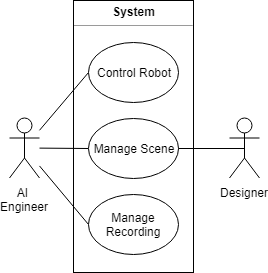
\includegraphics[width=6cm]{tex/img/ch04/UseCases_HighLevel_01.png}
\captionof{figure}{High-level Use-Cases}
\label{fig:use-cases-abstract}
\end{center}

The specific design of scenes and robots and the implementation of mutators depend on the scenario that the object-recognition software, that is to be trained, is used in: software run on cars should be trained using images generated in scenes that represent the environment the car is planned to be operated in and the robots used in these scenes should be modeled so they closely represent the car the software is to be run on, considering physical attributes (such as the car's shape, surfaces and size), behaviour (including acceleration, weight and steering)  and sensor-placement, where visual sensors such as camera are of the highest importance to the process of generating images.

%\begin{center}
%\noindent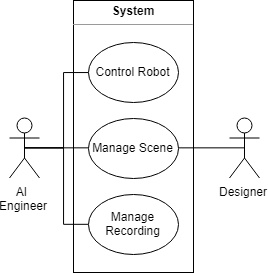
\includegraphics[width=6cm]{tex/img/ch04/Use_Cases_06.png}
%\captionof{figure}{Abstract use-Cases}
%\label{fig:use-cases-abstract}
%\end{center}

%////////////////////////////////////////////////
\section{User Interaction}
The use-cases shown in \ref{fig:use-cases-abstract} require further refinement before specific components can be deduced from them.

\paragraph{Use-Case "Control Robot"} \acs{AI} engineers may want to take control of robots and maneuver them in scenes by accelerating, decelerating and steering them or resetting them in case of being unable to maneuver (this may be the case when the robot was flipped or trapped between objects). While operating in manual mode, this can also be used to evaluate the usefulness (e.g. mobility) of certain robot-bodies in certain environments, presuming that the scene and robot behave like they would in real-life. This may require physics simulation for gravity and collision detection, and mechanics simulation for kinematics. Also, manual control of robots requires a careful choice of input devices: \acs{AI} engineers should use input devices allow for precise and true to original control of robots. For instance, a combination of a steering wheel and gas and break pedals closely resembles the control options present in cars whereas joysticks can be mapped to control torque of continuous tracks used on tracked vehicles.

\paragraph{Use-Case "Manage Recording"} \acs{AI} engineers need to be able to start and stop automatic capturing of records. As records are effectively pairs of images and a list of labels, both elements of these pairs must be provided by the system: it needs to feature a component that captures images from a camera held by a robot in a scene. To populate records with labels the system needs to provide a component that identifies classifiers in the captured images.

\paragraph{Use-Case "Manage Scene"}
[TBD]
% Designer: import assets (3d meshes, textures, mapshttps://www.google.com/search?q=bausteinsicht&source=lnms&tbm=isch&sa=X&ved=0ahUKEwiEmcHXkfffAhW6isMKHezUAwIQ_AUIDigB&biw=1642&bih=919#imgrc=HlRZw2laH-EwLM:) of scene and robots, add & configure mutators
% AI engineer: edit mutators/waypoints

\begin{center}
\noindent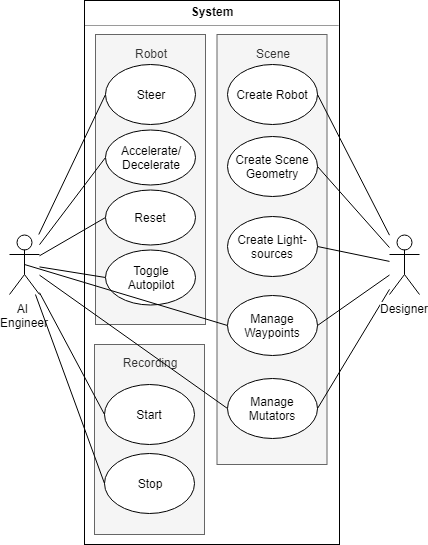
\includegraphics[width=10cm]{tex/img/ch04/UseCases_Fine_01.png}
\captionof{figure}{Refined Use-Cases [TBD]}
\label{fig:use-cases}
\end{center}

%////////////////////////////////////////////////
\section{Components}
Figure \ref{fig:use-cases} shows the high-level use-cases described in both modes, implicating the need for three high-level features (\ref{fig:component-diagram}): one that will be used to control robots (\textit{RobotController}), one that manages capturing records (\textit{Recording}) and one that allows designers to set up scenes (\textit{SceneManagement}).

\begin{center}
\noindent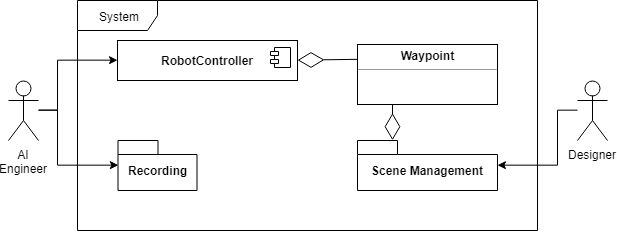
\includegraphics[width=12cm]{tex/img/ch04/ComponentDiagram01.png}
\captionof{figure}{High-level component diagram}
\label{fig:component-diagram}
\end{center}

Refining the \textit{Recording}-package yields two components (\ref{fig:component-diagram-recording}): \textit{RenderingController} shall generate images from a robot's perspective and save them while \textit{ImageLabeller} adds \textit{Labels} to the images and saves them. [TBD]

\begin{center}
\noindent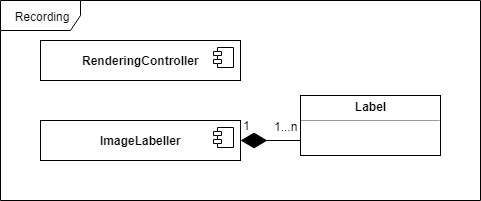
\includegraphics[width=12cm]{tex/img/ch04/ComponentDiagram_Recording03.png}
\captionof{figure}{Recording-package}
\label{fig:component-diagram-recording}
\end{center}

The \textit{SceneManagement}-package also contains two components (\ref{fig:component-diagram-scenemanagement}): the \textit{MutationManager} manages the aforementioned mutators in scenes (e.g. triggering and resetting mutations), the \textit{WaypointManager} holds a list of paths consisting of multiple waypoints.

\begin{center}
\noindent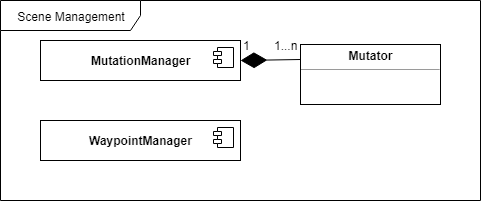
\includegraphics[width=12cm]{tex/img/ch04/ComponentDiagram_SceneManagement02.png}
\captionof{figure}{SceneManagement-package}
\label{fig:component-diagram-scenemanagement}
\end{center}


\section{Summary}
The concept is designed so that it is operating-system-, platform- and framework-agnostic. This results in an abstract concept that describes a basic architecture and abstract components.